
\documentclass[UTF8]{ctexart}
\usepackage{tikz,mathpazo}
\usetikzlibrary{shapes.geometric, arrows.meta}
\usepackage{flowchart}
\begin{document}
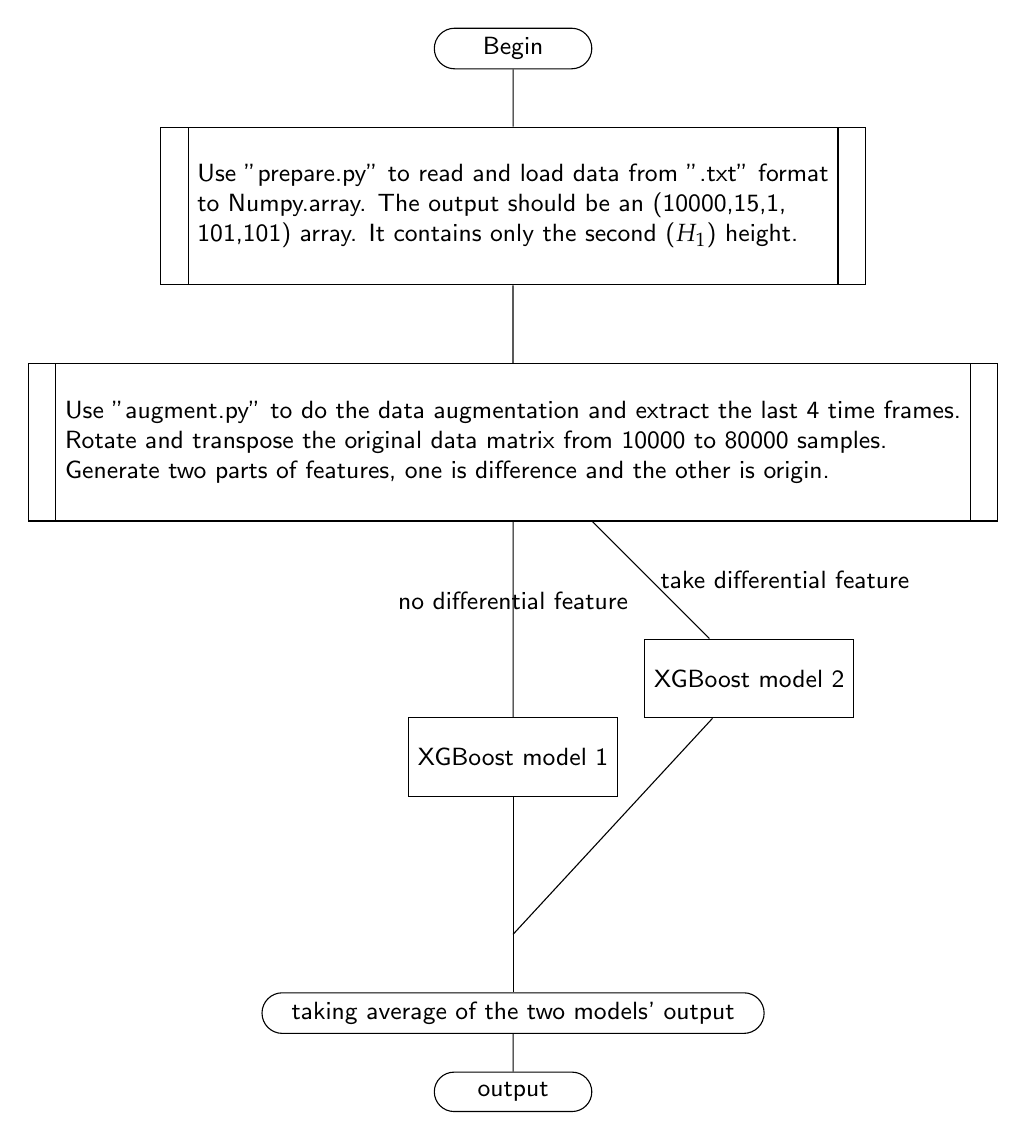
\begin{tikzpicture}[font={\sf \small}]
\def \smbwd{2cm}
\thispagestyle{empty}


\node (start) at (0,0.5) [draw, terminal,minimum width=\smbwd, minimum height=0.5cm] {Begin};
\node (getdata) at (0,-1.5) [draw, predproc, align=left,minimum width=\smbwd,minimum height=2cm] {Use "prepare.py" to read and load data from ".txt" format \\ to Numpy.array. The output should be an (10000,15,1, \\ 101,101) array. It contains only the second ($H_1$) height.}; 
\node (getdata2) at (0,-4.5) [draw, predproc, align=left,minimum width=\smbwd,minimum height=2cm] {Use "augment.py" to do the data augmentation and extract the last 4 time frames. \\ Rotate and transpose the original data matrix from 10000 to 80000 samples. \\ Generate two parts of features, one is difference and the other is origin.}; 
\node (storage) at (0,-8.5) [draw, process, minimum width=\smbwd, minimum height=1cm] {XGBoost model 1}; 
\node (process) at (3,-7.5) [draw, process, minimum width=\smbwd, minimum height=1cm] {XGBoost model 2}; 
\coordinate (point1) at (0,-10.75);
\node (end) at (0,-11.75) [draw, terminal,minimum width=\smbwd,minimum height=0.5cm] {taking average of the two models' output}; 
\node (output) at (0,-12.75) [draw, terminal,minimum width=\smbwd,minimum height=0.5cm] {output}; 

 %连接定义的形状,绘制流程图--表示垂直线,|表示箭头方向
\draw (start) -- (getdata);
\draw (getdata) -- (getdata2);
\draw (getdata2) -- node[anchor=west]{take differential feature}(process);
\draw (getdata2) -- node[above]{no differential feature}(storage);
\draw (process) -- (point1);
\draw (storage) -- (point1) -- (end);
\draw (end) -- (output);
\end{tikzpicture}
\end{document}
